% !TeX root = ../main.tex

\section{Approach}

This section presents the detailed design and implementation of \tool{}, our hierarchical framework for project-level Java to C++ code translation. We first provide an overview of the framework architecture, then describe each component in detail.

\begin{figure*}[h]
\centering

\includegraphics[width=\textwidth]{figures/architecture-overall.pdf}
\caption{Overall architecture of \tool{} showing the three-phase translation process.}
\label{fig:architecture-overview}
\end{figure*}

\subsection{Framework Overview}

Figure~\ref{fig:architecture-overview} illustrates the overall architecture of \tool{}. The framework adopts a macro-to-micro translation strategy that separates high-level structural design from low-level implementation details. The translation process consists of three main phases:

\begin{enumerate}
\item \textbf{Static Analysis Phase}: A custom Java parser tool extracts the project structure, including class hierarchies, method signatures, and call graph dependencies. This phase decomposes the codebase into a hierarchical graph representation that guides subsequent translation.

\item \textbf{Hierarchical Translation Phase}: The framework performs translation in two layers:
\begin{itemize}
\item \textit{Class-level translation}: For each Java class, interface, and enum, the LLM generates a translation scheme that maps Java language constructs to appropriate C++ patterns (e.g., interfaces to virtual base classes, exceptions to RAII patterns).
\item \textit{Method-level translation}: Methods are translated bottom-up according to the call graph, ensuring that callees are translated before their callers. This dependency-aware ordering enables context propagation, where already-translated code serves as reference for translating dependent methods.
\end{itemize}

\item \textbf{Validation and Repair Phase}: An autonomous compilation agent iteratively compiles the translated C++ code, analyzes errors, and applies fixes using LLM-generated suggestions. This phase continues until compilation succeeds or maximum attempts are reached.
\end{enumerate}

\subsection{Static Analysis and Graph Construction}

The first phase of \tool{} involves parsing the Java source code and extracting structural information necessary for guiding the translation process.

\subsubsection{Java Parser Tool}

We developed a custom Java parser tool (based on JavaParser)that processes Java source files and extracts:
\begin{itemize}
\item \textbf{Type declarations}: Classes, interfaces, enums, and their hierarchical relationships
\item \textbf{Method signatures}: Including parameter types, return types, and modifiers
\item \textbf{Field declarations}: Member variables with their types and access modifiers
\item \textbf{Import statements}: External dependencies required by each compilation unit
\end{itemize}

The parser integrates with \texttt{java-callgraph2}, a dependency analysis tool that extracts method call relationships.

This information is used to construct a dependency graph that determines the optimal translation order for methods.

\subsection{Hierarchical Translation Pipeline}

The translation pipeline include the translation of class-level and method-level code, each level is further divided into two steps.

\subsubsection{Class-Level Translation}

\paragraph{Scheme Generation} For each compilation unit (class, interface, enum .etc), the LLM generates a \textbf{translation scheme}—a high-level strategy document that specifies:

\begin{itemize}
\item \textbf{Type mapping}: How Java types map to C++ types (e.g., \texttt{ArrayList<T>} $\rightarrow$ \texttt{std::vector<T>}, \texttt{String} $\rightarrow$ \texttt{std::string})
\item \textbf{External dependencies}: External dependencies that can't directly be translated (e.g., third-party libraries, types in Java standard library that can't directly be mapped)
\item \textbf{Refactoring scheme}: Structural changes needed to accommodate C++ idioms (e.g., Strategy for replacing Java's garbage collection; replacing Java's exception handling; converting Java's generics to C++ templates)
\end{itemize}

\paragraph{Header Translation} Using the generated scheme, the LLM translates each compilation unit to C++ header (.h file). The translation handles:

\begin{itemize}
\item Class declaration.
\item Field declarations with proper C++ types
\item Method declarations using translated signatures
\end{itemize}

\begin{figure*}
  \centering
  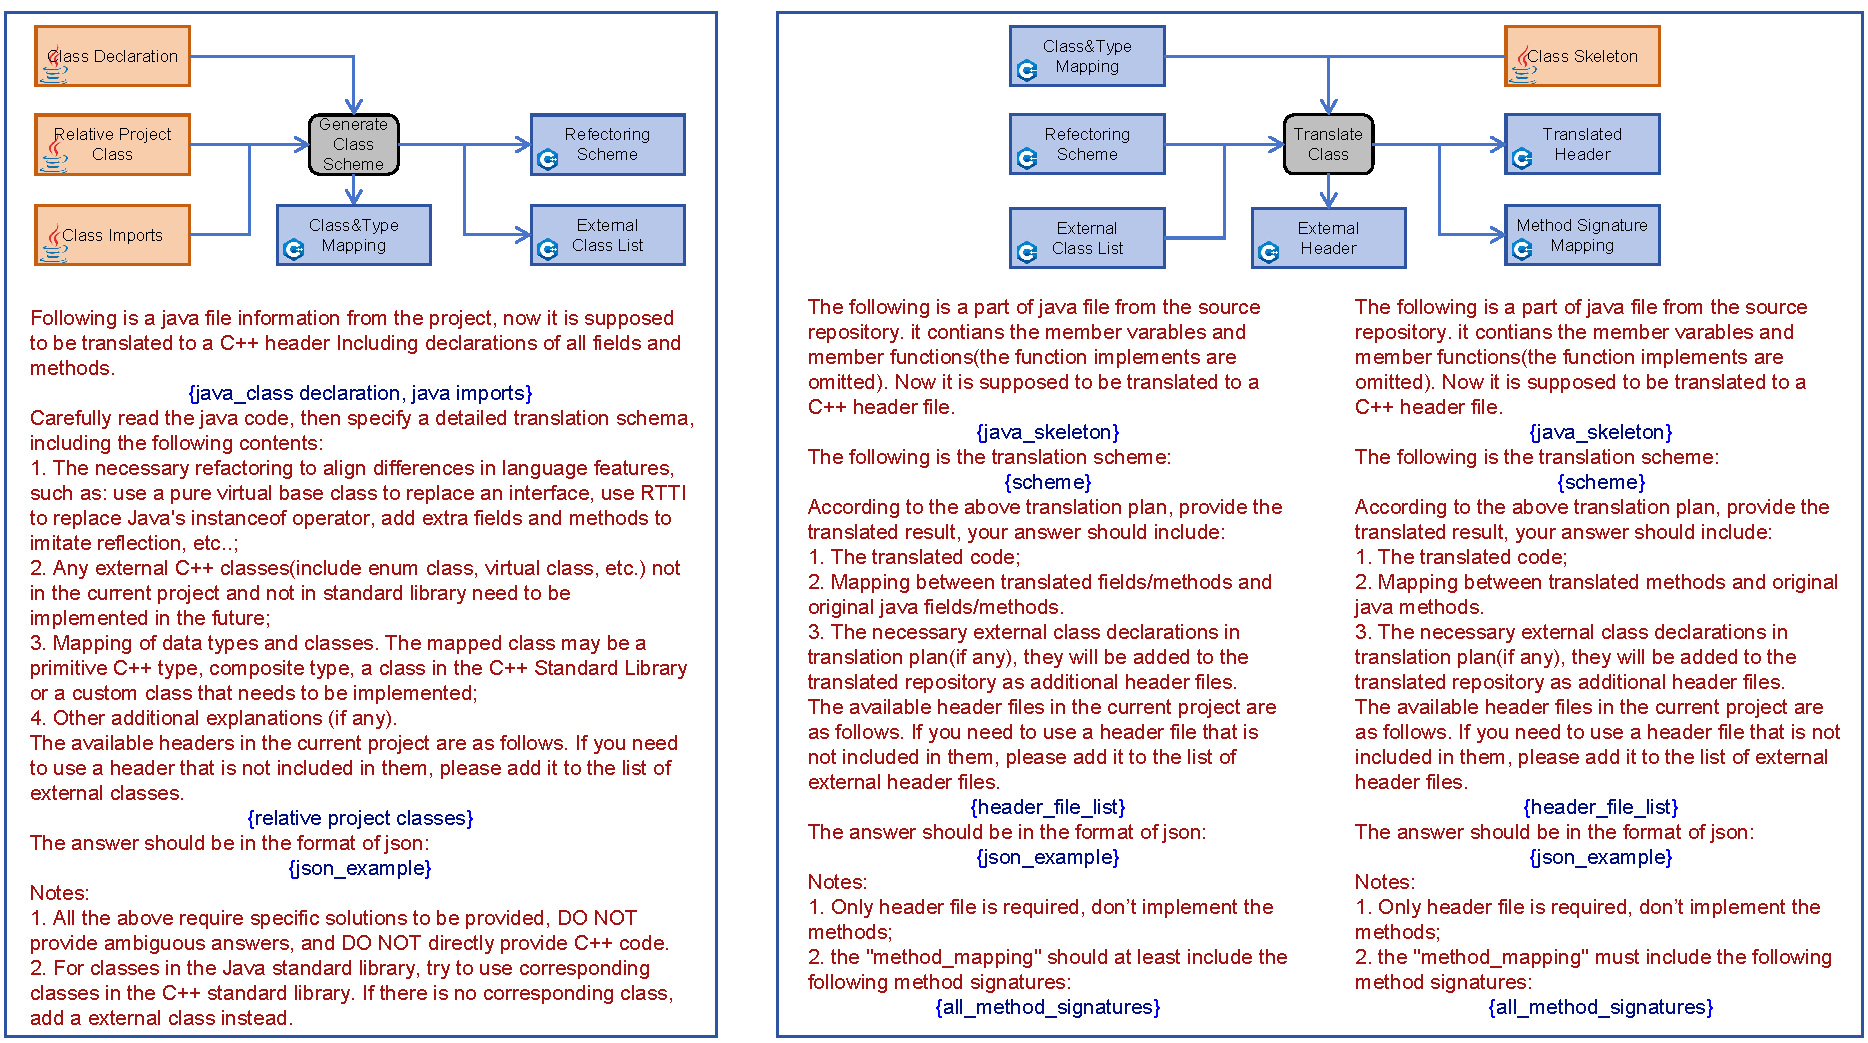
\includegraphics[width=\textwidth]{figures/class_translation.pdf}
  \caption{class translation prompts and data flow.}
  \label{fig:class-translation}
\end{figure*}

\subsubsection{Method-Level Translation}

\paragraph{Scheme Generation} For each Method, the LLM generates a detailed translation scheme that includes:
\begin{itemize}
\item \textbf{Functionality summary}: What the method does
\item \textbf{Implementation strategy}: How to achieve the same behavior in C++
\item \textbf{Context requirements}: Which already-translated methods to reference
\item \textbf{Exception handling}: How to convert Java checked exceptions to C++ error handling
\end{itemize}

The bottom-up order ensures that when generating a method's scheme, all its callees have already been translated and are available as context.

\paragraph{Method Translation} Methods are translated layer by layer. For each method, the LLM receives:
\begin{itemize}
\item The original Java method code
\item The method's translation scheme
\item The translated code of all callees (from previous layers)
\item The translated Header for context
\end{itemize}

This context-rich prompting reduces hallucination by providing concrete examples of how similar constructs were translated elsewhere in the project.

\begin{figure*}
  \centering
  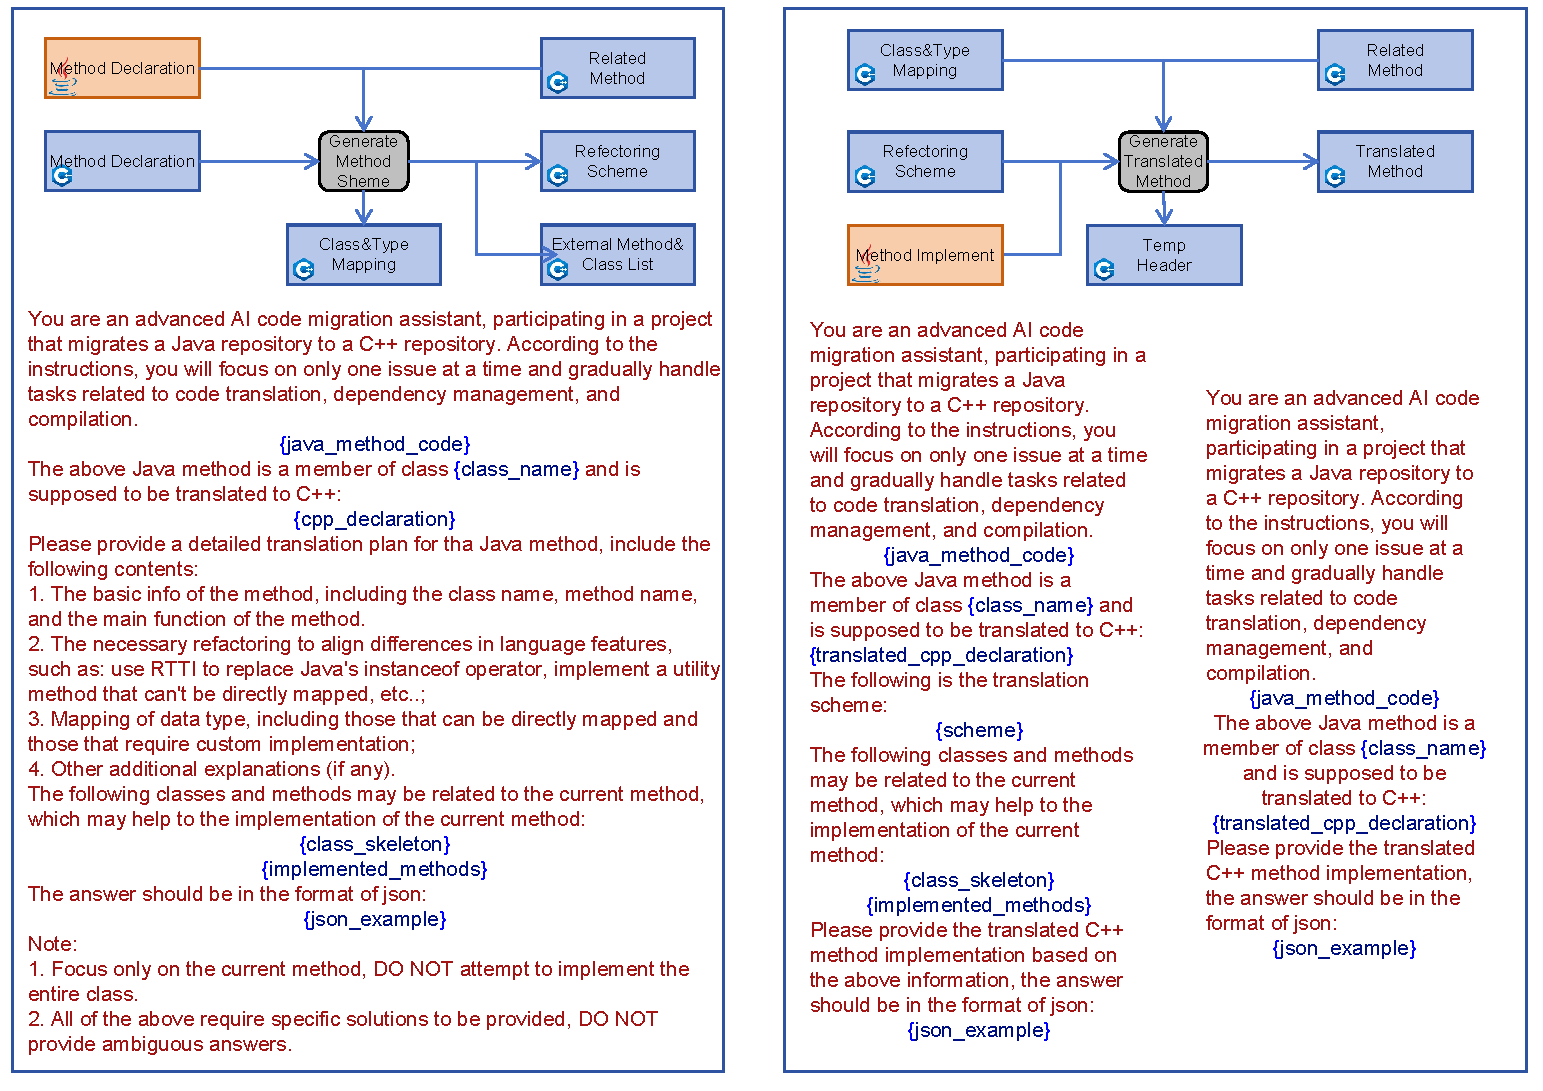
\includegraphics[width=\textwidth]{figures/method_translation.pdf}
  \caption{method translation prompts and data flow.}
  \label{fig:method-translation}
\end{figure*}

\subsection{Validation and Repair}


\subsection{Key Design Features}

\subsubsection{Bottom-Up Translation Order}

\subsubsection{Dual-Pass Translation}

Each translation unit (Header and Method) undergoes two passes:
\begin{enumerate}
\item \textbf{Scheme Pass}: High-level planning without generating code
\item \textbf{Code Pass}: Implementation guided by the scheme
\end{enumerate}

The two-pass approach separates planning from execution, allowing the LLM to reason about strategy before committing to implementation details.
